\subsection*{Example model (model ID: nn)}
The Example model (fig.~\ref{fig:nn_schematic}) is used in the MARRMoT User Manual to show how to create a new MARRMoT model from scratch \citep{Knoben2018b}. It has 3 stores and 7 parameters ($UZ_{max}$, $c_{rate}$, $p_{rate}$, $k_{lz}$, $ \alpha$, $k_{g}$, $d$). The model aims to represent:

\begin{itemizecompact}
\item Saturation excess from the upper zone;
\item Two-way interaction between upper and lower zone through percolation and capillary rise;
\item A split between fast subsurface flow and groundwater recharge from the lower zone;
\item Slow runoff from the groundwater;
\item Triangular routing of combined surface and subsurface flows.
\end{itemizecompact}

\subsubsection*{File names}
\begin{tabular}{@{}ll}
Model:  &m\_nn\_example\_7p\_3s \\
Parameter ranges: &m\_nn\_example\_7p\_3s\_parameter ranges \\
\end{tabular}

% Equations
\subsubsection*{Model equations}

% Model layout figure
{ 																	% This ensures it doesn't warp text further down
\begin{wrapfigure}{l}{6cm}
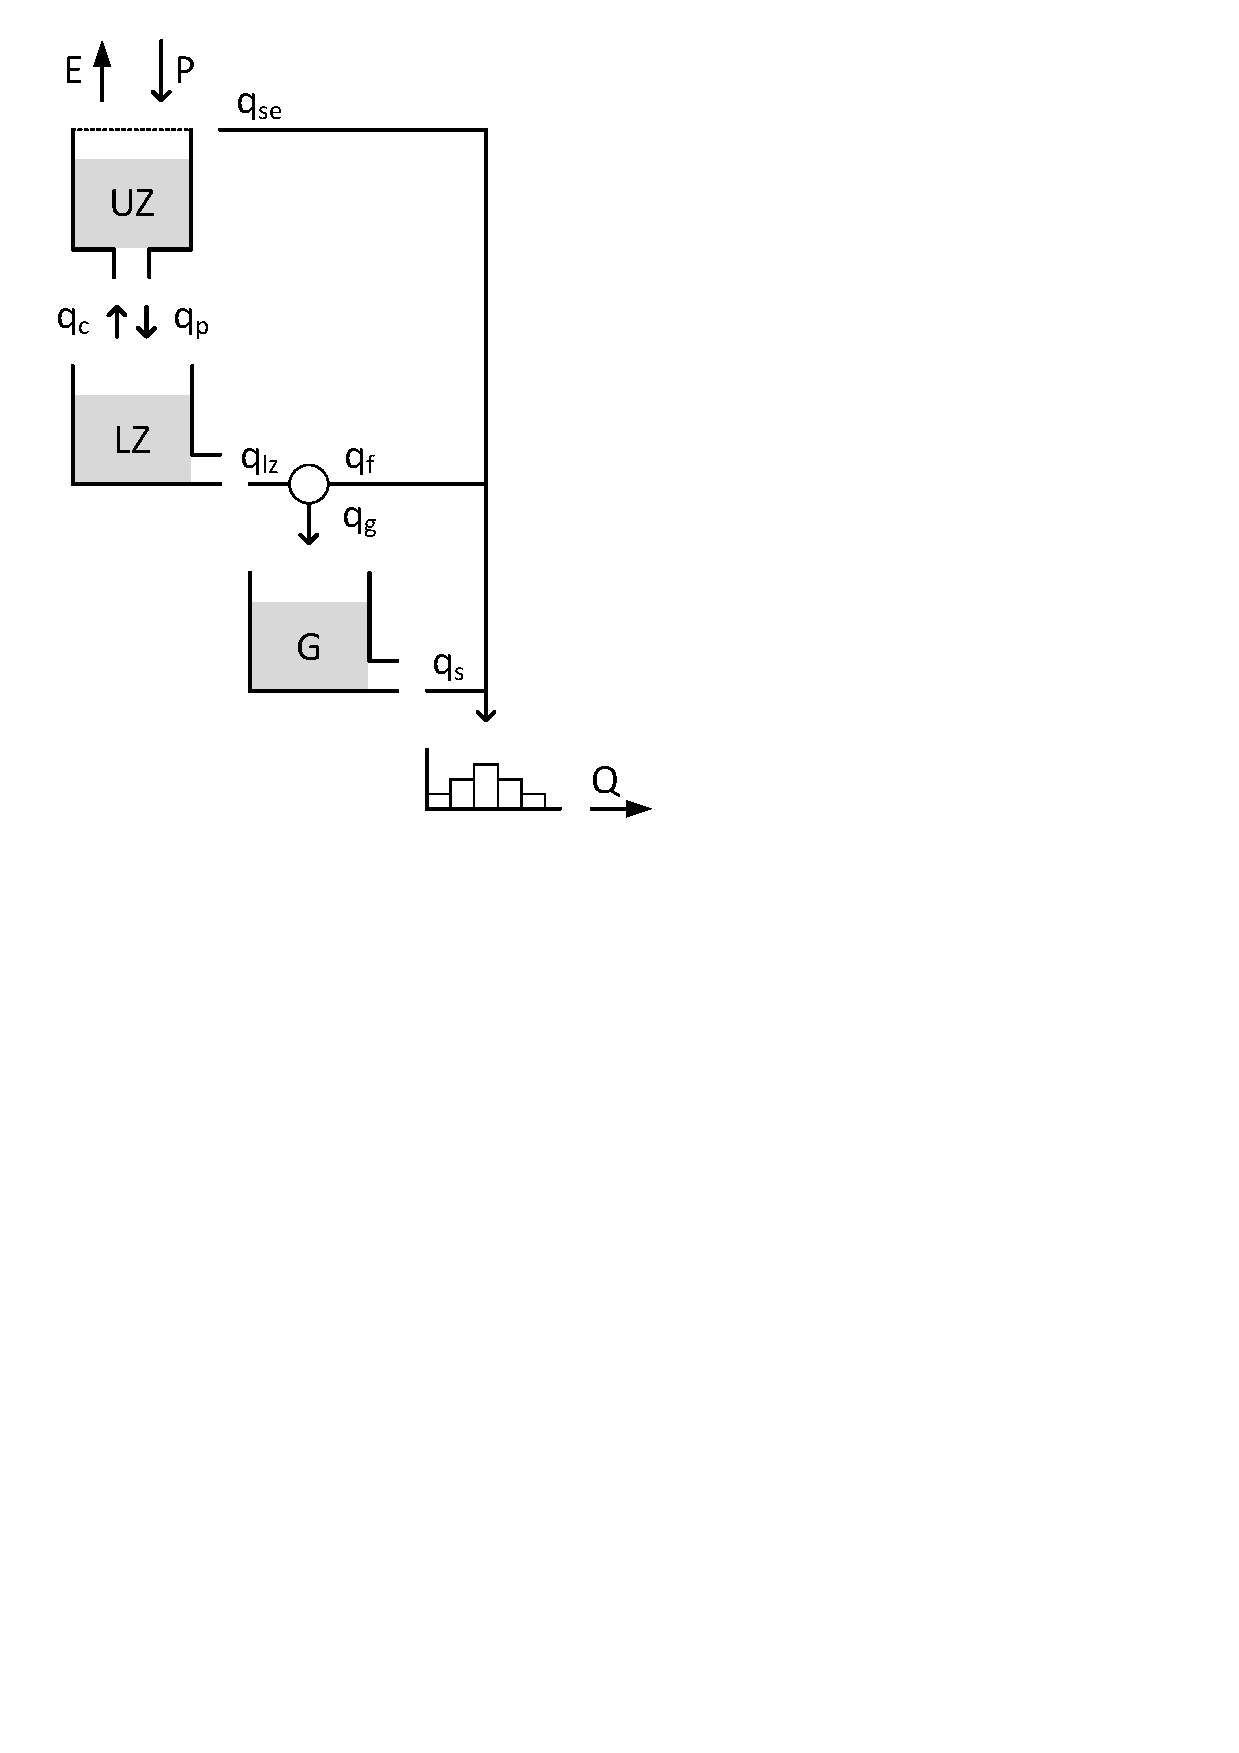
\includegraphics[trim=1cm 16cm 7cm 1cm,width=7cm,keepaspectratio]{./files/nn_schematic.pdf}
\caption{Structure of the Example model} \label{fig:nn_schematic}
\end{wrapfigure}

\begin{align}
	\frac{dUZ}{dt} &= P+ q_c -E-q_{se}-q_p \\
	E &= E_p*\frac{UZ}{UZ_{max}}\\
	q_c &= c_{rate}\left(1-\frac{UZ}{UZ_{max}}\right)\\
	q_{se} &= \begin{cases}
		P, &\text{if } UZ = UZ_{max}\\
		0, &\text{otherwise}\\
	\end{cases}	\\
	q_p &= p_{rate}
\end{align}

Where $UZ$ [mm] is the current storage in the upper zone, refilled by precipitation $P$ $[mm/d]$ and capillary rise $q_c$ $[mm/d]$ and drained by evaporation $E$ $[mm/d]$, percolation $q_p$ $[mm/d]$ and saturation excess $q_{se}$ $[mm/d]$.
Evaporation occurs at the potential rate $E_p$ scaled by the current storage in $UZ$ compared to maximum storage $UZ_{max}$ [mm].
Capillary rise occurs at a maximum rate $c_{rate}$ $[mm/d]$ if $UZ=0$ and decreases linearly if not.
Saturation excess flow only occurs when $UZ$ is at maximum capacity.
Percolation occurs at a constant rate $p_{rate}$ $[mm/d]$.

} % end of wrapfigure fix

\begin{align}
	\frac{dLZ}{dt} &= q_p - q_c - q_{lz}\\
	q_{lz} &= k_{lz}*LZ 
\end{align}

Where $LZ$ [mm] is the current storage in the lower zone, refilled by percolation $q_p$ $[mm/d]$ and drained by capillary rise $q_c$ $[mm/d]$ and outflow $q_{lz}$ $[mm/d]$.
Outflow has a linear relation with storage through time parameter $k_{lz}$ $[d^{-1}]$.

\begin{align}
	\frac{dG}{dt} &= q_g-q_s\\
	q_g &= \alpha*q_{lz} \\
	q_s &= k_g*G
\end{align}
  
Where $G$ [mm] is the current groundwater storage, refilled by recharge $q_g$ $[mm/d]$ and drained by slow flow $q_s$ $[mm/d]$.
Recharge is a fraction $\alpha$ [-] of outflow from the lower zone.
Outflow has a linear relation with storage through time parameter $k_{g}$ $[d^{-1}]$.
Saturation excess $q_{se}$, interflow $q_f$ and slow flow $q_s$ are combined and routed with a triangular Unit Hydrograph with time base $d$ [d] to give outflow $Q$ $[mm/d]$.

% Parameters
\subsubsection*{Parameter overview}
% Table generated by Excel2LaTeX from sheet 'Sheet1'
\begin{table}[htbp]
  \centering

    \begin{tabular}{lll}
    \toprule
    Parameter & Unit  & Description \\
    \midrule
    $UZ_{max}$ & $mm$    & Maximum soil moisture storage \\
    $c_{rate}$ & $mm~d^{-1}$ & Capillary rise rate \\
    $p_{rate}$ & $mm~d^{-1}$ & Percolation rate \\
    $k_{lz}$ & $d^{-1}$ & Lower zone runoff coefficient \\
    $\alpha$ & $-$     & Fraction of lower zone runoff that becomes recharge \\
    $k_g$   & $d^{-1}$ & Groundwater runoff coefficient \\
    $d$     & $d$     & Unit Hydrograph time base \\
    \bottomrule
    \end{tabular}%
  \label{tab:addlabel}%
\end{table}%

